% Capítulo 6: grafo não dirigido (amizades) e grafo dirigido (seguidores).
\documentclass[border=4pt]{standalone}
\usepackage[utf8]{inputenc}
\usepackage[T1]{fontenc}
% Estilo comum das figuras de grafos (capítulo 6).
% Estilo comum das figuras de árvores (capítulo 5).
\usepackage{tikz}
\usetikzlibrary{arrows.meta, positioning, calc}
\definecolor{navy}{RGB}{23,45,80}
\definecolor{laranja}{RGB}{250,110,29}
\definecolor{cinzalogo}{RGB}{107,114,126}
\tikzset{
  vertice/.style={circle, draw=navy, line width=0.9pt, fill=laranja!12, minimum size=8mm,
                  inner sep=0pt, font=\sffamily\small},
  destaque/.style={vertice, fill=laranja!45, draw=laranja},
  apagado/.style={vertice, dashed, draw=cinzalogo, fill=white, text=cinzalogo},
  arvore/.style={level distance=12mm, edge from parent/.style={draw=navy, line width=0.9pt}},
  rotulo/.style={font=\sffamily\small\bfseries, text=navy},
  legenda/.style={font=\sffamily\scriptsize, text=cinzalogo},
  setanova/.style={-{Stealth[length=2.2mm]}, laranja, line width=1.3pt},
}

\tikzset{
  aresta/.style={draw=navy, line width=0.9pt},
  arestaforte/.style={draw=laranja, line width=2.6pt},
  peso/.style={font=\sffamily\scriptsize, fill=white, inner sep=1.2pt, text=navy},
  arco/.style={-{Stealth[length=2.4mm]}, draw=navy, line width=0.9pt, shorten >=0.5pt},
  dist/.style={font=\sffamily\scriptsize\bfseries, text=laranja},
}
% Posições do grafo de exemplo (cidades A a F).
\newcommand{\posicoes}{%
  \coordinate (pA) at (0,0);
  \coordinate (pB) at (2.4,1.4);
  \coordinate (pC) at (2.4,-1.4);
  \coordinate (pD) at (5.2,1.4);
  \coordinate (pE) at (5.2,-1.4);
  \coordinate (pF) at (7.6,0);
}
\newcommand{\arestasexemplo}{A/B/4, A/C/2, B/C/1, B/D/5, C/D/8, C/E/7, D/E/2, D/F/6, E/F/3}
% \grafoexemplo{arestas destacadas, ex.: A/C, C/B}{estilo dos vértices}
\newcommand{\grafoexemplo}[2]{%
  \posicoes
  \foreach \a/\b/\p in \arestasexemplo { \draw[aresta] (p\a) -- (p\b); }
  \foreach \a/\b in {#1} { \draw[arestaforte] (p\a) -- (p\b); }
  \foreach \a/\b/\p in \arestasexemplo { \path (p\a) -- node[peso] {\p} (p\b); }
  \foreach \v in {A,B,C,D,E,F} { \node[#2] (\v) at (p\v) {\v}; }
}

\begin{document}
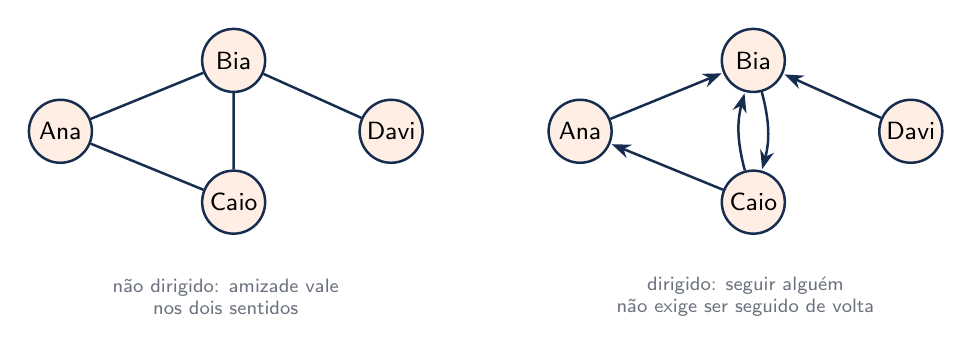
\begin{tikzpicture}
  % não dirigido
  \node[vertice] (ana) at (0,0) {Ana};
  \node[vertice] (bia) at (2.2,0.9) {Bia};
  \node[vertice] (caio) at (2.2,-0.9) {Caio};
  \node[vertice] (davi) at (4.2,0) {Davi};
  \draw[aresta] (ana) -- (bia) (ana) -- (caio) (bia) -- (caio) (bia) -- (davi);
  \node[legenda, align=center] at (2.1,-2.1) {não dirigido: amizade vale\\nos dois sentidos};

  % dirigido
  \begin{scope}[xshift=6.6cm]
    \node[vertice] (ana2) at (0,0) {Ana};
    \node[vertice] (bia2) at (2.2,0.9) {Bia};
    \node[vertice] (caio2) at (2.2,-0.9) {Caio};
    \node[vertice] (davi2) at (4.2,0) {Davi};
    \draw[arco] (ana2) -- (bia2);
    \draw[arco] (caio2) -- (ana2);
    \draw[arco] (bia2) to[bend left=15] (caio2);
    \draw[arco] (caio2) to[bend left=15] (bia2);
    \draw[arco] (davi2) -- (bia2);
    \node[legenda, align=center] at (2.1,-2.1) {dirigido: seguir alguém\\não exige ser seguido de volta};
  \end{scope}
\end{tikzpicture}
\end{document}
